\section{Question 5\label{section:ex5}}

\begin{figure}[htp]
    \centering
    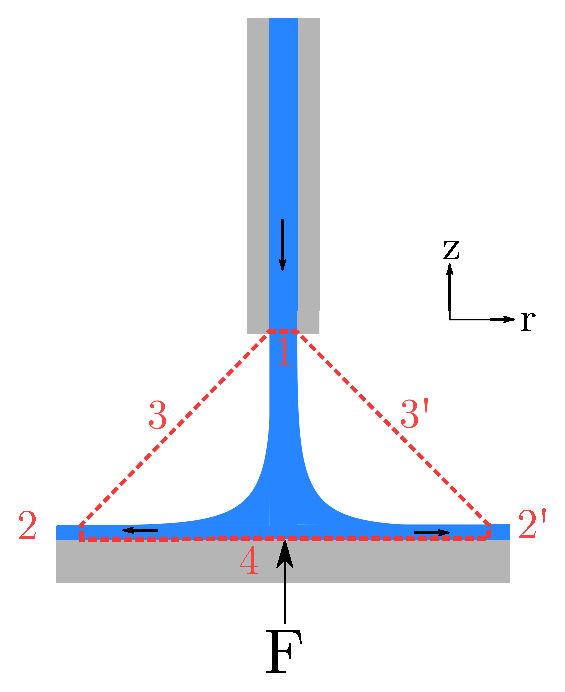
\includegraphics[width = 0.5\linewidth]{images/FigureExo5.eps}
    \caption{Représentation simplifiée de la configuration du jet en représentation 2D}
    \label{fig:config_exo5}
\end{figure}

On considère la configuration représentée à la figure \ref{fig:config_exo5} en 2D où un jet uniforme sort d'un tube de section $A_{in}$ à vitesse constante $- v_z \vec{e}_z$. Cet jet heurte une plaque plane (circulaire en 3D) sur lequel il se réoriente radialement. Du fait de cette réorientation, le jet exerce sur la plaque une force $\vec{F}_{jet \rightarrow plaque}$, ou de manière équivalente (3\up{e} loi de Newton), la plaque exerce une force $\vec{F}_{plaque \rightarrow jet} = - \vec{F}_{jet \rightarrow plaque} = F \vec{e}_z$ pour simplifier. \\

On fera l'hypothèse que le problème est invariant par rotation. Cela implique notamment que le jet se réoriente dans toutes les directions uniformément sur la plaque (direction $r$). Ainsi, on aura : $\iint_{2 \cup 2'} \vec{u}_{(\vec{r})}dS = \vec{0}$.\\

D'autre part, on choisit un volume de contrôle invariant par rotation dont une représentation est proposée en pointillés rouges sur la figure \ref{fig:config_exo5}. Ce volume est \emph{fixe} par rapport au référentiel de l'observateur ainsi que du jet. Sa surface peut être décomposée comme suit :
\begin{itemize}
    \item L'entrée $1$, de surface $A_{in} = \pi R_{in}^2$ et de normale sortante $\vec{e}_z$ où le fluide entre normalement avec une vitesse moyenne $-v_z \vec{e}_z$
    \item la surface de sortie $2$ (et $2'$ dans la vue place), section de cylindre vertical, dont la normale est selon $\vec{e}_r$
    \item La surface $3$ (et $3'$ en 2D) de forme conique mais dont le flux de toute quantité est nul
    \item La surface $4$ qui reprend la frontière de la plaque avec une forme de disque. Les lignes de courant de vitesse étant tangente à cette surface, les flux à travers $4$ seront également nuls
\end{itemize}

\medskip

On effectue alors un bilan de quantité de mouvement $\rho \vec{u}$ sur ce volume $V$ en utilisant le théorème général de Liebnitz. Ainsi, d'après le principe fondamental de la dynamique :

\begin{equation}
    \frac{d}{dt} \iiint_V \rho \vec{u} ~ dV = \vec{F}_{ext \rightarrow V} = \vec{F}
\end{equation}


D'autre part

\begin{equation}
    \frac{d}{dt} \iiint_V \rho \vec{u} dV = \underbrace{\iiint_V \cancel{\frac{\partial \rho \vec{u}}{\partial t}}dV}_{\textnormal{Hypothèse régime stationnaire}} + \iint_{\partial V} \rho \vec{u} \otimes \vec{u}.\vec{dS} 
\end{equation}

On peut décomposer le terme de flux $\iint_{\partial V} \rho \vec{u} \otimes \vec{u}.\vec{dS}$ sur les différentes parties du contour du volume précédemment décrit :

\begin{itemize}
    \item Sur l'entrée $1$ : 
    \begin{equation}
        \iint_{\partial V \cap 1} \rho \vec{u} \otimes \vec{u}.\vec{dS} = \iint_{\partial V \cap 1} \rho (-v_z) \vec{e}_z \otimes \underbrace{\left( -v_z \vec{e}_z \right).\left(dS \vec{e}_z\right)}_{\textnormal{Scalaire } ~ -v_z dS} = \rho A_{in} v_z^2 \vec{e}_z
    \end{equation}
    
    \item Sur la surface de sortie $2$, on a déjà conclu par symétrie que l'intégrale de toute quantité vectorielle elle-même symétrique doit s'annuler (cf. l'intégrale d'une fonction impaire sur un intervalle centré en zéro). Plus mathématiquement :
    
    \begin{equation}
        \iint_{\partial V \cap 2} \rho \vec{u} \otimes \vec{u}.\vec{dS} = \iint_{\partial V \cap 2} \rho u_r \vec{e}_r \otimes \left(u_r \vec{e}_r\right) . \left(dS \vec{e}_r \right) = \int_0^h dz \rho u_r^2 \underbrace{\int_0^{2\pi} d\theta \vec{e}_r}_{= 0 ~ \textnormal{par symétrie}} = \vec{0}
    \end{equation}
    \item Sur les surfaces $3$ et $4$, le flux étant nul, les intégrales le sont également :
    \begin{equation}
        \iint_{\partial V \cap (3 \cup 4)} \rho \vec{u} \otimes \underbrace{\vec{u}.\vec{dS}}_{= 0 } = \vec{0}
    \end{equation}
\end{itemize}

En fusionnant les trois parties de l'intégrale, on obtient :

\begin{equation}
    \vec{F} = \rho A_{in} v_z^2 \vec{e}_z = W_l v_z \vec{e}_z
\end{equation}

où $W_l$ est le débit massique $W_l = \iint_A \rho \vec{u}.\vec{dS} = A \dot{m}$. D'un point de vue physique, cela fait sens et peut être interprété comme un débit de quantité de mouvement (davantage qu'un effet d'accélération). En effet, entre $t$ et $t+dt$, le jet éjecte une masse $dm = W_l dt$ à la vitesse $v_z$ soit une variation infinitésimale de quantité de mouvement $dp = d(mv) = dm . v + \cancel{m. dv} = W_l dt \times v_z$. On retrouve alors $F = \frac{dp}{dt} = W_l v_z$.\\

On pourrait généraliser la configuration du jet à un cas plus général où le jet s'échappe dans des directions non orthogonales au jet initial. Cela ajoute une contribution au terme de force. Ainsi dans certaines turbines de type Pelton, le jet peut repartir "en arrière", ce qui a tendance à augmenter l'effort produit. Au contraire, si le jet est appliqué sur un plan incliné, il peut seulement être dévié, ce qui a pour effet de réduire l'effort $F$. Enfin on peut également généraliser ce principe à des systèmes sans plaque, par exemple la propulsion de fusées.\\
